\chapter{相关工作}
\label{cha:related_work}
本文研究的内容包含了深度学习、多任务学习与自然语言处理三个主题,这里首先阐述这些主题之间的联系,接着分别介绍它们各自的相关概念与研究进展,最后介绍了三者交叉的一些重要研究工作。

我们利用深度学习与多任务学习来解决自然语言处理中的问题,具体的,即在深层神经网络中使用多任务学习来获得文本的泛化表示。从这一角度来看,深度学习与多任务学习是我们的工具,而自然语言处理为我们的应用场景。同时,深度学习与多任务学习都可以归为机器学习问题,而他们二者又有交叉,如图~\ref{fig:ml_dl_mtl}~所示。

\begin{figure}[htb]
	\centering
	\begin{tikzpicture}[scale=0.8]
	\draw (-4,3) rectangle (4,-3);
	\draw[draw = black] (-1.5,0) circle (2);
	\draw[draw = black] (1.5,0) circle (2);
	\node at (-2.8,2.5) {机器学习};
	\node at (-2,0) {深度学习};
	\node at (2,0) {多任务学习};
	\end{tikzpicture}
	\caption{机器学习、深度学习、多任务学习的关系}
	\label{fig:ml_dl_mtl}
\end{figure}

\section{深度学习}
\label{sec:dl}
近年来,深度学习(Deep Learning)发展十分迅速,在人工智能的很多子领域上取得了巨大成功,如语音识别\cite{DBLP:conf/asru/MikolovDPBC11}\cite{DBLP:conf/apsipa/LiHYW13}、计算机视觉\cite{DBLP:journals/cacm/KrizhevskySH17}\cite{DBLP:journals/pami/FarabetCNL13}\cite{DBLP:conf/nips/TompsonJLB14}、自然语言处理\cite{DBLP:journals/jmlr/CollobertWBKKK11}\cite{DBLP:conf/emnlp/BordesCW14}\cite{DBLP:conf/acl/JeanCMB15}\cite{DBLP:conf/nips/SutskeverVL14}等。

从要研究的问题来看,深度学习属于机器学习的一个分支,都是研究如何从有限个样例中通过某种算法总结出一般性规律或模式,并将其应用到新的未知数据上去。例如,通过机器学习或深度学习算法,可以根据历史病例总结出症状与疾病之间的规律,当遇到新的病人时可以利用算法总结出来的规律来帮助判断这个病人得了什么疾病\footnote{例子来源:《神经网络与深度学习》,邱锡鹏,\url{https://nndl.github.io}}。

同时,深度学习又与机器学习有很大的不同。从模型的构成来说,深度学习模型一般更加复杂,参数量更多。由于数据从输入到输出需要经过多个线性或非线性组件,信息传递路径较长,因此被称作深度学习。深度学习模型的一个最典型代表就是人工神经网络(Artificial Neural Network,ANN),下面简称神经网络。神经网络是一种受人脑神经系统启发的复杂数学模型,由神经元以及它们之间的连接组成。通过这些神经元的加工,原始数据从底层特征开始经过一道道加工逐渐得到抽象的高层语义特征。

总的来说,神经网络可以被看做一个包含大量参数的复合函数,该函数描述了输入和输出之间的复杂关系,因此可以被用于处理很多模式识别任务,如语音识别、图像识别等。形式化地,神经网络可以这样描述:
\begin{equation}
	y = \mathcal{F}(\mathbf{x} \mid \theta).
\end{equation}
其中,函数~$\mathcal{F}$~受参数~$\theta$~控制。

给定包含大量样例的集合,参数~$\theta$~可以通过随机梯度下降等优化算法得到,求解参数的优化过程就被称为\emph{学习过程},通过学习得到的参数被称为\emph{可学习参数},常简称为参数。还有一部分不可以被学习的参数,例如神经网络的层数,被称为\emph{超参数},意为控制参数的参数,超参数通常根据经验指定或根据实验效果来确定。

前面提到,参数学习需要一个包含大量样例的集合,该集合就是\emph{数据集}。在有监督学习中,每个样例一般包含输入~$\mathbf{x}$~和输出~$y$,输出也常被称为标签。其中,输入一般为一个向量,向量的每一个维度表示了样本的一个属性;输出一般为一个标量。包含~$n$~个样例的集合~$\mathcal{D} = \{ \mathbf{x}_i, y_i \}_{i=1}^n$~就是数据集。在实际使用时,数据集通常被划分为训练集、验证集(也叫开发集)和测试集。其中,用训练集来让算法学习参数,用验证集来调整算法的超参数,用测试集来衡量模型的优劣。

给定数据集~$\mathcal{D}$~和模型结构,即~$\mathcal{F}$的形式,优化算法可以得到参数~$\theta$~进而确定模型~$\mathcal{F}(\theta)$. 下面介绍一种简单的前馈神经网络结构:多层感知机(Multi-Layer Perceptron, MLP)。一个单隐层的MLP可以记作~$\mathcal{F}(\mathbf{x} \mid \theta) = \mathbf{W}_2(f(\mathbf{W}_1\mathbf{x} + b_1))+b_2$,其中参数~$\theta = \{ \mathbf{W}_1, b_1, \mathbf{W}_2, b_2 \}$,函数~$f(\cdot)$~为非线性激活函数,如ReLU. 多层感知机的结构如图~\ref{fig:mlp}~所示,为简单起见,图中省略了偏置项~$b_1, b_2$.

\begin{figure}[htb]
	\def\layersep{2.5cm}
	\centering
	\begin{tikzpicture}[shorten >=1pt,->,draw=black!50, node distance=\layersep]
	\tikzstyle{every pin edge}=[<-,shorten <=1pt]
	\tikzstyle{neuron}=[circle,fill=black!25,minimum size=17pt,inner sep=0pt]
	\tikzstyle{input neuron}=[neuron, fill=white!50, draw=black];
	\tikzstyle{output neuron}=[neuron, fill=white!50, draw=black];
	\tikzstyle{hidden neuron}=[neuron, fill=lightgray!50, draw=black];
	\tikzstyle{annot} = [text width=4em, text centered]
	
	% Draw the input layer nodes
	\foreach \name / \y in {1,...,4}
	% This is the same as writing \foreach \name / \y in {1/1,2/2,3/3,4/4}
	\node[input neuron, pin=left:$x_{\y}$] (I-\name) at (0,-\y) {};
	
	% Draw the hidden layer nodes
	\foreach \name / \y in {1,...,5}
	\path[yshift=0.5cm]
	node[hidden neuron] (H-\name) at (\layersep,-\y cm) {};
	
	% Draw the output layer node
	\node[output neuron,pin={[pin edge={->}]right:$y$}, right of=H-3] (O) {};
	
	% Connect every node in the input layer with every node in the
	% hidden layer.
	\foreach \source in {1,...,4}
	\foreach \dest in {1,...,5}
	\path (I-\source) edge (H-\dest);
	
	% Connect every node in the hidden layer with the output layer
	\foreach \source in {1,...,5}
	\path (H-\source) edge (O);
	
	% Annotate the layers
	\node[annot,above of=H-1, node distance=1cm] (hl) {隐藏层};
	\node[annot,left of=hl] {输入层};
	\node[annot,right of=hl] {输出层};
	\end{tikzpicture}
	\caption{多层感知机}
	\label{fig:mlp}
\end{figure}

随着深度学习的发展,神经网络的结构也变得日益多样和复杂。上面的多层感知机属于全连接前馈网络,而前馈网络的另一典型代表就是在计算机视觉中被广泛使用的\emph{卷积神经网络}(Convolutional Neural Network, CNN),它与全连接网络的区别在于权重共享和局部连接。除前馈网络外,还有一类网络称为反馈网络,因为反馈网络的神经元可以接收来自本身的反馈信号,从而具备一定的记忆能力,因此也被称为记忆网络。反馈网络的一种典型代表就是\emph{循环神经网络}(Recurrent Neural Network, RNN),它在自然语言处理中得到了广泛应用。另外,近年来\emph{图神经网络}(Graph Neural Network, GNN)因其在处理图结构数据上的优势也得到了迅速发展。

深度学习能够成功的重要原因在于其强大的特征表示能力。在传统的机器学习中,通常需要人为地构造数据特征,再训练一个学习算法来总结这些构造出来的特征输入与输出之间的关系。例如,在文本分类任务中,传统机器学习的做法一般是利用词袋模型或TF-IDF来构造文本特征,再将其作为支持向量机等分类器的输入来进行分类。而在深层神经网络中,算法自动学习原始数据的特征表示,数据从输入到输出的过程~$\mathbf{x}\to \mathcal{F} \to y$~可以人为地划分为两个阶段:\emph{表示学习}和\emph{预测}。所谓表示,就是神经网络中间隐层的状态,上文中MLP的中间隐层就可以当作某种浅层表示;而预测,比如分类或回归,一般是在上一层得到的特征表示的基础上进行简单变换得到易于预测的任务特定表示。因此,深度学习又可以看作是一种表示学习,而深度学习的成功也证明了学到好的特征表示的重要意义。

\section{多任务学习}
\label{sec:mtl}
在机器学习中,我们通常关心模型在某个任务上的某个指标,并通过在某个数据集上训练单个模型或一组集成模型来达成此目标。事实上,有时我们可以同时利用其他数据集甚至其他任务来联合训练模型,从而进一步提升性能,这种方法就是\emph{多任务学习}(Multi-Task Learning, MTL)。

从定义上来说,多任务学习就是一种归纳转移(Inductive Transfer)方法,通过利用包含在相关任务训练信号中的领域特定信息来提升模型的泛化能力\cite{Caruana1997}。在机器学习中,给定训练集,存在多个假设能够解释训练数据,这些假设构成的空间被称为假设空间,里面的一个假设就对应了一个模型。不同的机器学习算法倾向于选择不同的假设,这种选择偏好被称为归纳偏置(Inductive Bias)。直观上,多任务学习使得算法倾向于选择一种能够同时解释多个任务的假设,也即引入了多个任务的归纳偏置。从表示学习的角度看,这样能够同时适用于多个任务的表示就是泛化的表示。图~\ref{fig:mtl_int}~较为直观地给出了多任务学习的一种解释。

\begin{figure}[htb]
	\centering
	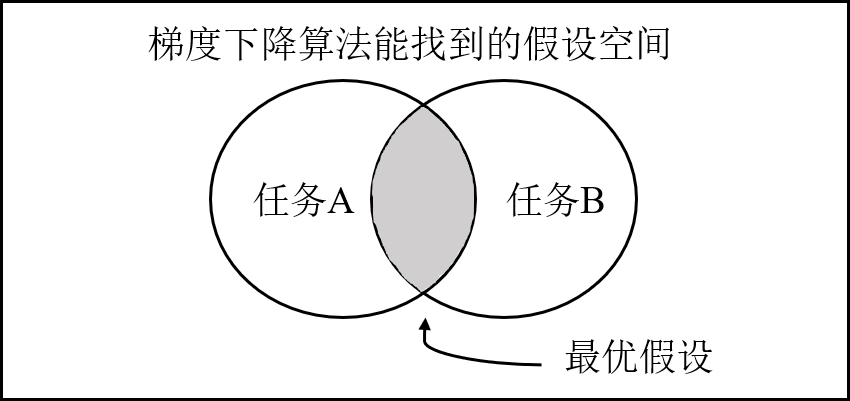
\includegraphics[scale=0.55]{mtl_int.png}
	\caption{多任务学习的一种直观解释}
	\label{fig:mtl_int}
\end{figure}

关于多任务学习为何有效,除了上面的解释(归纳偏置)之外,Caruana还给出了几种合理的解释\cite{Caruana1997}:

\begin{itemize}
	\item \textbf{数据增强(Statistical data amplification)} 由于多个任务的数据集通常是不同的,使用多个相关任务对同一个模型进行训练相当于增大了训练数据量。
	\item \textbf{特征选择(Attribute selection)} 如果任务噪声较大,或者数据高维而数据量有限,模型很难分辨相关特征和无关特征,而多任务学习可以帮助模型选出相关特征,因为这些特征通常在多个任务中是共用的。也就是说,其他任务为模型选择特征提供了额外的证据。
	\item \textbf{窃听(Eavesdropping)} 存在某些特征对于任务 $A$ 易于学习,而对于任务 $B$ 则难以学习。通过多任务学习,模型可以在执行任务 $B$ 时使用任务 $A$ 学到的特征。
\end{itemize}

在深度学习之前,多任务学习已经被应用在线性模型、核方法、决策树、多层感知机等传统机器学习算法上,有大量的研究集中在稀疏正则化\cite{DBLP:conf/nips/ArgyriouEP06}\cite{DBLP:conf/colt/LouniciPTG09}以及学习任务之间的关系\cite{DBLP:journals/jmlr/EvgeniouMP05}\cite{DBLP:conf/nips/JacobBV08}上。

随着深度学习的发展,多任务学习开始应用在深层神经网络中,并在自然语言处理\cite{DBLP:conf/icml/CollobertW08}、计算机视觉\cite{DBLP:conf/cvpr/MisraSGH16}、语音识别\cite{DBLP:conf/icassp/DengHK13}、药物设计\cite{DBLP:journals/corr/RamsundarKRWKP15}等众多应用场景中取得了成功。同时,多任务学习作为一种模型无关的方法,在卷积神经网络\cite{DBLP:conf/icml/CollobertW08}\cite{DBLP:conf/cvpr/MisraSGH16}、循环神经网络\cite{DBLP:conf/ijcai/LiuQH16}、图网络\cite{liu2018multi}上都可以应用。

然而,无论是在传统机器学习算法上还是在深层神经网络上,多任务学习的核心观点都在于知识共享。如何为特定任务和学习算法设计合适的共享模式一直是多任务学习的重要问题。从多任务学习的应用方式来看,可以大概分为下面四种共享模式\cite{book:nndl}:

\begin{itemize}
	\item \textbf{硬共享模式}:让不同任务的模型共享一些公用模块(比如神经网络的低层)来提取一些通用特征表示,然后再针对每个不同的任务设置一些私有模块(比如神经网络的高层)来提取任务特定的特征表示。
	\item \textbf{软共享模式}:不显式地设置共享模块,但每个任务都可以“窃取”其他任务的模型学习到的特征表示。窃取的方式多种多样,比如可以直接使用其它任务的隐状态,也可以使用注意力机制或门控机制来选取有用的特征。
	\item \textbf{分层共享模式}:一般神经网络中不同层抽取的特征类型不同。底层一般抽取一些低级的局部特征,高层抽取一些高级的抽象语义特征。因此如果多任务学习中不同任务也有级别高低之分,那么一个合理的共享模式是让低级任务在底层输出,高级任务在高层输出。
	\item \textbf{共享-私有模式}:一个更加分工明确的方式是将共享模块和任务特定(私有)模块的职责分开。共享模块捕捉一些跨任务的共享特征,而私有模块只捕捉和特定任务相关的特征。最终的表示由共享特征和私有特征共同构成。
\end{itemize}
四种共享模式如图~\ref{fig:mtl_archs}~所示。

\begin{figure}[htb]
	\centering
	
	\subfloat[硬共享模式]{
		\centering
		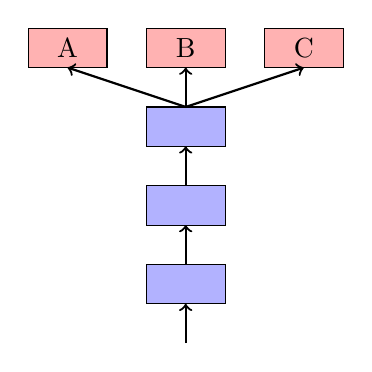
\begin{tikzpicture}
		\begin{scope} [fill opacity = .3]
		\draw [->, thick] (0,0) -- (0, 0.5);
		\draw [fill=blue, draw = black] (-0.5,1) rectangle (0.5, 0.5);
		\draw [->, thick] (0, 1) -- (0, 1.5);
		\draw [fill=blue, draw = black] (-0.5,2) rectangle (0.5, 1.5);
		\draw [->, thick] (0, 2) -- (0, 2.5);
		\draw [fill=blue, draw = black] (-0.5,3) rectangle (0.5, 2.5);
		\draw [fill=red, draw = black] (-2,4) rectangle (-1, 3.5);
		\draw [fill=red, draw = black] (-0.5,4) rectangle (0.5, 3.5);
		\draw [fill=red, draw = black] (1,4) rectangle (2, 3.5);
		\draw [->, thick] (0, 3) -- (-1.5, 3.5);
		\draw [->, thick] (0, 3) -- (0, 3.5);
		\draw [->, thick] (0, 3) -- (1.5, 3.5);
		\end{scope}
		\node at (-1.5, 3.75) {A};
		\node at (0, 3.75) {B};
		\node at (1.5, 3.75) {C};
		
		\end{tikzpicture}
	}
	\quad
	\subfloat[软共享模式]{
		\centering
		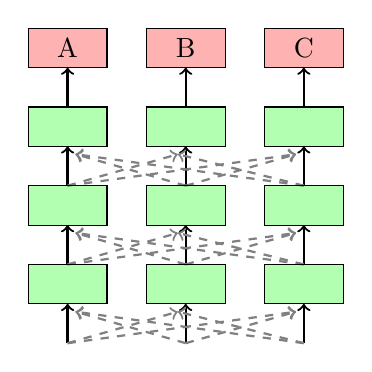
\begin{tikzpicture}
		\begin{scope} [fill opacity = .3]
		\draw [->, thick] (-1.5,0) -- (-1.5, 0.5);
		\draw [->, thick, gray, dashed] (-1.5,0) -- (-.1, 0.4);
		\draw [->, thick, gray, dashed] (-1.5,0) -- (1.4, 0.4);
		
		\draw [->, thick] (-1.5, 1) -- (-1.5, 1.5);
		\draw [->, thick, gray, dashed] (-1.5, 1) -- (-.1, 1.4);
		\draw [->, thick, gray, dashed] (-1.5, 1) -- (1.4, 1.4);
		
		\draw [->, thick] (-1.5, 2) -- (-1.5, 2.5);
		\draw [->, thick, gray, dashed] (-1.5, 2) -- (-.1, 2.4);
		\draw [->, thick, gray, dashed] (-1.5, 2) -- (1.4, 2.4);
		
		\draw [->, thick] (-1.5, 3) -- (-1.5, 3.5);
		
		\draw [fill=green, draw = black] (-2,1) rectangle (-1, 0.5);
		\draw [fill=green, draw = black] (-2,2) rectangle (-1, 1.5);
		\draw [fill=green, draw = black] (-2,3) rectangle (-1, 2.5);
		\draw [fill=red, draw = black] (-2,4) rectangle (-1, 3.5);
		
		\draw [->, thick] (0,0) -- (0, 0.5);
		\draw [->, thick, gray, dashed] (0,0) -- (-1.4, 0.4);
		\draw [->, thick, gray, dashed] (0,0) -- (1.4, 0.4);
		
		\draw [->, thick] (0, 1) -- (0, 1.5);
		\draw [->, thick, gray, dashed] (0, 1) -- (-1.4, 1.4);
		\draw [->, thick, gray, dashed] (0, 1) -- (1.4, 1.4);
		
		\draw [->, thick] (0, 2) -- (0, 2.5);
		\draw [->, thick, gray, dashed] (0, 2) -- (-1.4, 2.4);
		\draw [->, thick, gray, dashed] (0, 2) -- (1.4, 2.4);
		
		\draw [->, thick] (0, 3) -- (0, 3.5);
		
		\draw [fill=green, draw = black] (-0.5,1) rectangle (0.5, 0.5);
		\draw [fill=green, draw = black] (-0.5,2) rectangle (0.5, 1.5);
		\draw [fill=green, draw = black] (-0.5,3) rectangle (0.5, 2.5);
		\draw [fill=red, draw = black] (-0.5,4) rectangle (0.5, 3.5);
		
		\draw [->, thick] (1.5, 0) -- (1.5, 0.5);
		\draw [->, thick, gray, dashed] (1.5, 0) -- (-1.4, 0.4);
		\draw [->, thick, gray, dashed] (1.5, 0) -- (-.1, 0.4);
		
		\draw [->, thick] (1.5, 1) -- (1.5, 1.5);
		\draw [->, thick, gray, dashed] (1.5, 1) -- (-1.4, 1.4);
		\draw [->, thick, gray, dashed] (1.5, 1) -- (-.1, 1.4);
		
		\draw [->, thick] (1.5, 2) -- (1.5, 2.5);
		\draw [->, thick, gray, dashed] (1.5, 2) -- (-1.4, 2.4);
		\draw [->, thick, gray, dashed] (1.5, 2) -- (-.1, 2.4);
		
		\draw [->, thick] (1.5, 3) -- (1.5, 3.5);
		
		\draw [fill=green, draw = black] (1,1) rectangle (2, 0.5);
		\draw [fill=green, draw = black] (1,2) rectangle (2, 1.5);
		\draw [fill=green, draw = black] (1,3) rectangle (2, 2.5);
		\draw [fill=red, draw = black] (1,4) rectangle (2, 3.5);
		\end{scope}
		\node at (-1.5, 3.75) {A};
		\node at (0, 3.75) {B};
		\node at (1.5, 3.75) {C};
		
		\end{tikzpicture}
	}%
	\quad
	
	\subfloat[分层共享模式]{
		\centering
		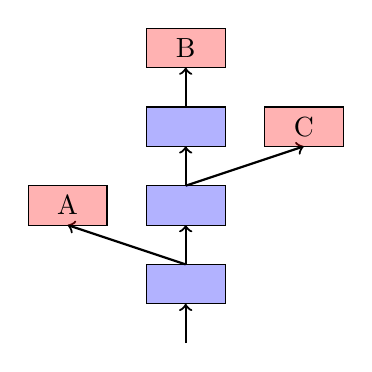
\begin{tikzpicture}
		\begin{scope} [fill opacity = .3]
		\draw [->, thick] (0,0) -- (0, 0.5);
		\draw [->, thick] (0, 1) -- (0, 1.5);
		\draw [->, thick] (0, 2) -- (0, 2.5);
		\draw [->, thick] (0, 3) -- (0, 3.5);
		\draw [->, thick] (0, 1) -- (-1.5, 1.5);
		\draw [->, thick] (0, 2) -- (1.5, 2.5);
		
		\draw [fill=blue, draw = black] (-0.5,1) rectangle (0.5, 0.5);
		\draw [fill=blue, draw = black] (-0.5,2) rectangle (0.5, 1.5);
		\draw [fill=blue, draw = black] (-0.5,3) rectangle (0.5, 2.5);
		
		\draw [fill=red, draw = black] (-0.5,4) rectangle (0.5, 3.5);
		\draw [fill=red, draw = black] (-2,2) rectangle (-1, 1.5);
		\draw [fill=red, draw = black] (1,3) rectangle (2, 2.5);
		\end{scope}
		\node at (-1.5, 1.75) {A};
		\node at (0, 3.75) {B};
		\node at (1.5, 2.75) {C};
		
		\end{tikzpicture}
	}
	\quad
	\subfloat[共享-私有模式]{
		\centering
		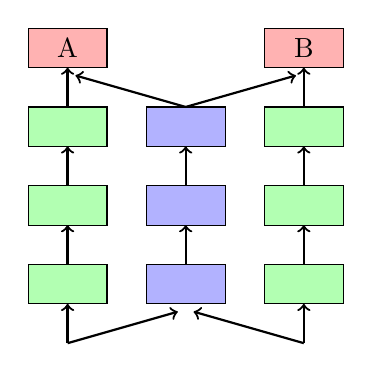
\begin{tikzpicture}
		\begin{scope} [fill opacity = .3]
		\draw [->, thick] (-1.5,0) -- (-1.5, 0.5);
		\draw [->, thick] (-1.5, 1) -- (-1.5, 1.5);
		\draw [->, thick] (-1.5, 2) -- (-1.5, 2.5);
		\draw [->, thick] (-1.5, 3) -- (-1.5, 3.5);
		
		\draw [fill=green, draw = black] (-2,1) rectangle (-1, 0.5);
		\draw [fill=green, draw = black] (-2,2) rectangle (-1, 1.5);
		\draw [fill=green, draw = black] (-2,3) rectangle (-1, 2.5);
		\draw [fill=red, draw = black] (-2,4) rectangle (-1, 3.5);
		
		\draw [->, thick] (-1.5,0) -- (-.1, .4);
		\draw [->, thick] (1.5,0) -- (.1, .4);
		\draw [->, thick] (0, 1) -- (0, 1.5);
		\draw [->, thick] (0, 2) -- (0, 2.5);
		\draw [->, thick] (0, 3) -- (-1.4, 3.4);
		\draw [->, thick] (0, 3) -- (1.4, 3.4);
		
		\draw [fill=blue, draw = black] (-0.5,1) rectangle (0.5, 0.5);
		\draw [fill=blue, draw = black] (-0.5,2) rectangle (0.5, 1.5);
		\draw [fill=blue, draw = black] (-0.5,3) rectangle (0.5, 2.5);
		
		\draw [->, thick] (1.5, 0) -- (1.5, 0.5);
		\draw [->, thick] (1.5, 1) -- (1.5, 1.5);
		\draw [->, thick] (1.5, 2) -- (1.5, 2.5);
		\draw [->, thick] (1.5, 3) -- (1.5, 3.5);
		
		\draw [fill=green, draw = black] (1,1) rectangle (2, 0.5);
		\draw [fill=green, draw = black] (1,2) rectangle (2, 1.5);
		\draw [fill=green, draw = black] (1,3) rectangle (2, 2.5);
		\draw [fill=red, draw = black] (1,4) rectangle (2, 3.5);
		\end{scope}
		\node at (-1.5, 3.75) {A};
		\node at (1.5, 3.75) {B};
		
		\end{tikzpicture}
	}
	
	\caption{多任务学习的几种常见共享模式}
	\label{fig:mtl_archs}
\end{figure}

\section{自然语言处理}
\label{sec:nlp}





\section{多任务自然语言处理}
\label{sec:mtl4nlp}
